\chapter{Funktionen}\label{chap:kommandos}

In diesem Kapitel werden alle Funktionalitäten des TGG Editors erklärt. Die Basis Funktionen, sind Funktionen, die so gut wie jeder gewöhnliche Editor unterstützt. Danach folgen die speziellen Funktionen des TGG Editors.

\section{Basis Funktionen}
\subsection{Copy/Paste}
Copy und Paste werden vom TGG Editor leider nicht unterstützt.

\subsection{Undo/Redo}
Während des Arbeitens mit dem Editor kann man jederzeit die einzelnen ausgeführten Schritte mit \emph{Undo}\index{Undo} rückgängig machen und mit \emph{Redo}\index{Redo} wiederholen.
\begin{enumerate}
	\item Wähle per Rechtsklick das Kontextmenü und dort \emph{Undo} oder \emph{Redo}.
	\item Wähle in der Menüleiste \texttt{Edit}$\rightarrow$\texttt{Undo} und \texttt{Edit}$\rightarrow$\texttt{Redo}.
	\item Drücke den Button 
\includegraphics[height=0.5cm]{undo_icon} für \emph{Undo} und 
\includegraphics[height=0.5cm]{redo_icon} für \emph{Redo}.
	\item Oder per Shortcut: \texttt{Strg+z} für \emph{Undo} und \texttt{Strg+y} für \emph{Redo}.
\end{enumerate}

\subsection{Property View}
\begin{wrapfigure}{l}{8cm}
	\centering
	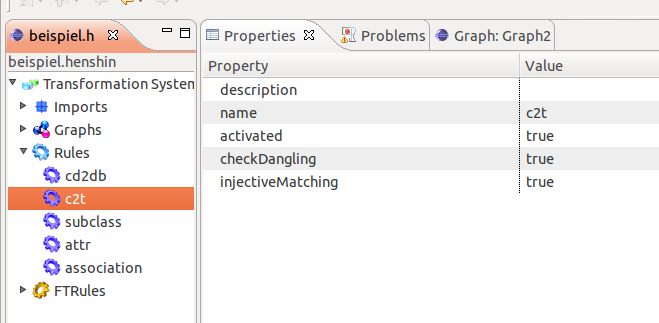
\includegraphics[width=7cm]{property_view}
	\caption{Property View}
	\label{fig:property_view}
\end{wrapfigure}
Namen und Typen können im \emph{Property View}\index{Property View} editiert werden. Zunächst muss man den \emph{Property View} wie folgt öffnen: Man wählt im Hauptmenü \texttt{Window}$\rightarrow$\texttt{Show View}$\rightarrow$\texttt{Other} oder benutzt den Shortcut \texttt{Shift+Alt+q q}. Es erscheint ein Fenster. Dort wählt man im Ordner \texttt{General} den Eintrag \texttt{Properties}. Es erscheint ein neuer View wie in Abbildung \ref{fig:property_view} dargestellt.

\subsection{Direct Edit}
Man hat die Möglichkeit die Namen von Objekten im oben beschriebenen Property View zu verändern oder einfach mit dem \emph{Direct Edit}\index{Direct Edit} Feature. Dazu muss man das gewünscht Objekt markieren und dann noch einmal auf den Namenstext klicken. Dann erscheint der Text wie in Abbildung ... zu sehen ist. Jetzt kann man einen Namen der Wahl eingeben und auf der Tastatur mit \texttt{Enter} abschließen oder das Objekt wieder deselektieren. 

\subsection{Delete}
Sobald ein Objekt ausgewählt ist kann man mit der Taste \texttt{Entfernen} das Objekt löschen. Alternativ kann man aber auch mit einem Rechtsklick auf das Objekt klicken und aus dem Kontextmenü den Eintrag \textit{Delete}\index{Delete} ausführen.

\section{Tree View}
Der \emph{Tree View}\index{Tree View} ist eine baumartige Ansicht des gesamten Projektes, des \emph{Transformation System}. Man findet hier die Ordner \emph{Imports}, \emph{Graphs}, \emph{Rules} und \emph{FTRules}.

\subsection{Imports}
Im Ordner Imports\index{Imports} erscheinen die importierten EMF Modelle für Source, Correspondence und Target. Diese Modelle sollen die einzelnen Teile einer TGG beschreiben. Sie sind die Metamodelle. Das Metamodell für Source beschreibt demnach die Quellsprache. Das Metamodell für Target beschreibt entsprechend die Zielsprache. Wie wir wissen benötigt man außerdem noch einen Correspndence Teil, der die beiden anderen beiden Teile verbindet. 

\subsubsection{Ein EMF Modell importieren}
Um ein solches Metamodell zu importieren muss es zunächst in den Workspace importiert werden. Gehe dann wie folgt vor: 
\begin{enumerate}
	\item Mit einem Rechtsklick auf den Ordner Imports kann die entsprechende Action, entweder $Import Source, Correspondece$ oder $Target$ aufgerufen werden.
	\item Wähle über \textit{Workspace...} die entsprechende ECORE-Datei für Source, Correspondence oder Target.
\end{enumerate}
Sobald ein Metamodell importiert ist, kann man in im Graph- und Rule View Instanzen des Metamodells erstellen.

\subsection{Graphs}
Im Ordner Graphs\index{Gaph} werden die Graphen, die das Transformation System enthält, angezeigt. Durch einen Doppleklick auf einen Graphen öffnet sich der Graph View. Klappt man im Tree View den Graphen auf so erscheinen alle Komponenten, die ein Graph enthält, Nodes und Edges. Nodes werden in folgendem Schema angezeigt: \texttt{Name:Typ}. Der \texttt{Name} ist der zugewiesene Node Name. \texttt{Typ} ist einer der Typen aus einem der Metamodelle (entweder Source, Correspondence oder Target). Klappt man die auch die Nodes auf so erscheinen die Edges eines Nodes. Die werden in folgendem Schema angezeigt \texttt{EdgeTyp: fromTyp->toTyp}. Der \texttt{EdgeTyp} ist einer der Typen einer Edge aus einem der Metamodelle. Da die Edges im Henshin Modell gerichtet sind, gibt es einen Typen, \texttt{fromType}, für den Source-Node und einen Typen,\texttt{toType}, für den Target-Node.

\subsubsection{Einen neuen Graphen erstellen}
Um einen neuen Graph zu erstellen gehe wie folgt vor:
\begin{enumerate}
	\item Über einen Rechtsklick auf den Ordner \textit{Graphs} lässt sich die Aktion \textit{Create\  Graph} ausführen.
	\item Wähle einen Namen für den Graphen.
\end{enumerate}


\subsection{Rules}
Im Ordner Rules\index{Rule} werden die Rules, die das Transformation System enthält, angezeigt. Ein weiteres aufklappen einer Rule funktioniert nicht. Die einzelnen Komponenten einer Rule werden demnach nicht angezeigt. Durch anklicken mit einem Doppelklick einer Rule öffnet sich die Rule View.

\subsubsection{Eine neue Rule erstellen}
Um eine neue Rule zu erstellen gehe wie folgt vor:
\begin{enumerate}
	\item Über einen Rechtsklick auf den Ordner \textit{Graphs} lösst sich die Aktion \textit{Create\ Rule} ausführen.
	\item Wähle einen Namen für die neue Rule.
\end{enumerate}

Über Rechtsklick im Tree View kann man noch weitere Aktionen ausführen. Diese Aktionen stehen aber in näherem Zusammenhang mit den Views, die im folgenden Abschnitten beschrieben werden. Sie sind meistens auch zusätzlich in der Toolbar der View zu erreichen. Aus diesem Grund werden auch die Aktionen in den entsprechenden Abschnitten für die View beschrieben.

\section{Graph View}\index{Graph View}
Im \emph{Graph View} werden Tripelgraphen einer TGG dargestellt und können editiert werden. Die Zeichenfläche des Graph Views ist dreigeteilt. Der linke Teil für Source, der mittlere für Correspondence, der rechte für Target. Zusätzlich sind die Nodes der einzelnen Teile rot, blau und gelb eingefärbt.

\subsection{Palette}\index{Palette}
Die Palette bietet einige Tools, um den Graphen zu editieren.

\subsubsection{Select}\index{Select Tool}
\label{subsubsec:Graph_View-Select}
Das \emph{Select Tool} ist das standardmäßig ausgewählte Tool. Mit dem Select Tool kann man einzelne Objekte mit einem Klick auswählen. Man kann aber auch mehrere Objekte auswählen, indem man einen Kasten über die Objekte zieht. Alternativ kann man aber auch alle auszuwählenden Objekte anklicken während man \texttt{Shift} gedrückt hält. Das primär ausgewählte Objekt wird rot markiert, die sekundär gewählten Objekte werden grün markiert. Dies ist hilfreich, wenn man Mappings für eine NAC editiert.

\subsubsection{Node}\index{Node Tool}
\label{subsubsec:Graph_View-Node}
Das Tool mit dem man \emph{Nodes} zeichnen kann wird nicht direkt mit dem Namen Node angezeigt. Vielmehr existieren für je Source, Correspondence und Target Teil je eine Gruppe von Node Tools. Es wird nämlich nicht allgemein ein Node kreiert, sondern über die Auswahl des entsprechenden Tools wird ein Node \textit{mit einem bestimmten Typen} kreiert. Die einzelnen Tools haben den Namen der jeweiligen Typen. Hat man wie in unserem Beispiel\footnote{Siehe Abschnitt \ref{chap:Workflow}} den Typ \emph{Class} im importierten EMF Modell für den Source Teil, so heißt das Node Tool auch Class. Wenn man versucht einen Node, der eigentlich in den Source Teil gehört, in den Target Bereich zeichnen möchte, so ist dies nicht möglich. Der Mauszeiger verwandelt sich dann in ein Kreuz.

\subsection{Edge}\index{Edge Tool}
\label{subsubsec:Graph_View-Edge}
Mit dem \emph{Edge Tool} kann man Edges zwischen Nodes zeichnen. Man muss hierzu zuerst auf den Quell-Node klicken, danach auf den Ziel-Node. Falls mehr als ein Typ von Edges zwischen den Nodes existieren kann, öffnet sich ein Dialog zur Auswahl des Typen. Falls die Edge nicht gezeichnet werden kann, wird dies am Mauszeiger mit einem Verbotssymbol angezeigt.

\subsubsection{Attribute}\index{Attribute Tool}
\label{subsubsec:Graph_View-Attribute}
Wenn das \emph{Attribute Tool} ausgewählt ist, können Attribute erstellt werden. Dazu muss man auf einen Node klicken, zu welchem man das Attribut erstellen möchte. Daraufhin erscheint ein Dialog, indem man den Namen und den Wert des Attributes angeben kann.

\subsection{Toolbar}\index{Toolbar}
In der \emph{Toolbar} befinden sich Aktionen, die auf den gesamten Tripelgraphen ausgeführt werden können.

\subsubsection{Validate Graph}\index{Validate Graph}
Mit der Aktion Validate Graph kann man den Graphen auf seine EMF Konsistenz überprüfen. Falls die Überprüfung erfolgreich war, wird dies in einem Dialog angezeigt. Falls sie nicht erfolgreich war, werden die Fehler im Dialog angezeigt. Diese Aktion ist auch über das Kontextmenü im Tree View verfügbar, wenn man auf einen Graphen klickt.

\subsubsection{Execute FT Rules}\index{Execute FT Rules}
Mit dieser Aktion werden alle Forward Translation Rules\index{FT Rule}, die es im gesamten Transformation System gibt, ausgeführt. Nach der Ausführung wird überprüft, ob die Modelltransformation \emph{Source Consistent}\index{Source Consistent} war oder nicht. Die Nodes und Edges, die nicht übersetzt wurden, werden in der Meldung angezeigt. Außerdem werden die Regeln in ihrer Ausführungsreihenfolge angezeigt. Bisher kann diese Ausführungsreihenfolge vom Benutzer nicht verändert werden. Außerdem wird sie deterministisch gewählt. Das heißt, dass bei mehrfacher Ausführung der Aktion immer wieder die selbe Reihenfolge von FT Rules gewählt wird. Die Aktion ist ebenfalls über das Kontextmenü im Tree View verfügbar, wenn man auf eine Rule klickt.


\section{Rule View}\label{sec:ruleview}
Der Rule View\index{Rule View} ist genauso aufgebaut wie der Graph View, ist aber um einige Funktionen wie der NAC-Ansicht, einigen Palette Tools und Aktionen in der Toolbar erweitert worden. Er dient zur graphischen Erstellung von Regeln, welche später auf einen Graphen angewendet, oder zur Generierung von FT-Regeln verwendet werden können. Wir haben für den Rule View eine kompakte Art der Darstellung gewählt. Eine Rule einer TGG hat eine Graphen als linke Seite und einen Graphen als rechte Seite. Dies wird im Rule View allerdings dem Benutzer nur indirekt angezeigt. Man sieht erst einmal nur die rechte Seite. Das macht den Rule View viel übersichtlicher. Wenn man ein Element hinzufügt, wird automatisch ein Element für den Graphen der linken Seite und eines für den der rechten Seite erstellt und falls nötig wird noch ein Mapping zwischen den beiden Elementen erstellt. In unserem Rule View ist allerdings nur möglich Regeln zu erstellen, die Elemente hinzufügen (siehe Abschnitt \ref{subsubsec:Rule_View-++}). Hier kümmert sich der Editor automatisch um die rechte und linke Seite und die Mappings.

\subsection{Palette}\index{Palette}
Die Palette im Rule View wurde im Vergleich zum Graph View um die Tools ++ und Mapping erweitert. Die Palette-Tools Select (\ref{subsubsec:Graph_View-Select}), Node (\ref{subsubsec:Graph_View-Node}), Edge (\ref{subsubsec:Graph_View-Edge}), Attribute (\ref{subsubsec:Graph_View-Attribute}) verhalten sich wie in den verherigen Kapiteln beschrieben.

\subsubsection{++}
\label{subsubsec:Rule_View-++}
Mit dem ++\index{++ Tool} Tool ist es möglich Nodes und Edges als neu zu markieren. Dies sind dann die Elemente, die bei einer Regelanwendung in einem Graphen neu erstellt werden. Folglich kann dieses Tool auch nicht auf Elemente in der NAC angewendet werden. \\
Zu beachten ist, dass falsches Markieren zu invaliden Regeln führen kann.

\subsubsection{Mapping}\index{Mapping Tool}
\label{subsubsec:Rule_View-Mapping}
Mit dem Mapping Tool ist es möglich ein Mapping zwischen einem Node in einem NAC Graphen und einem Node im Regelgraphen zu erstellen. Dabei können Mapping nur zwischen Nodes aus einer NAC und einer Regel erstellt werden, vom gleichen Typen sind und nicht als neu gekennzeichnet sind. Beim Erstellen eines Mapping ist zu beachten, dass als erstes der Node im Regelgraphen gewählt werden muss (dieser ist dann als einziger Node im Rule View markiert) und anschließend der gewünschte Node im NAC Graphen. Ist eine Auswahl eines bestimmten Nodes nicht möglich wird dies mit einem Verbotssymbol am Mauszeiger kenntlich gemacht.

\subsection{Toolbar}\index{Toolbar}
Die Toolbar des Rule Views enthält Aktionen zur Generierung einer FT-Regel, zum Validieren und Ausführen der aktuellen Regel

\subsubsection{Generate FT Rule}
Die Aktion \emph{Generate FT Rule}\index{Generate FT Rule} löscht, wenn vorhanden, die zu der aktuellen Regel gehörende FT-Regel und generiert aus der aktuellen Regel eine FT-Regel. Die generierte Regel lässt sich dann in Tree Editor unter \emph{FT Rules}\index{FT Rule} finden.
Möchte man für alle erstellten Rules gleichzeitig die FT Rules erstellen, nutzt man mit Rechtsklick im Kontextmenü des Regelordners im Treeview die Aktion \emph{"Generate All FT Rules"}\index{Generate All FT Rules}.

\subsubsection{Validate Rule}
Mit der Aktion \emph{Validate Rule}\index{Validate Rule} wird die Regel auf ihre EMF Konsistenz\index{EMF Konsistenz} überprüft. Falls die Überprüfung erfolgreich war, wird dies in einem Dialog angezeigt. Falls sie nicht erfolgreich war, werden die Fehler im Dialog angezeigt. Diese Aktion ist auch über das Kontextmenü im Tree View verfügbar, wenn man mit einem Rechtsklick auf eine Rule klickt.

\subsubsection{Execute Rule}
Die Aktion \emph{Execute Rule}\index{Execute Rule} für die Rule auf einem gewünschten Graphen aus. Sind mehrere Graphen im System registriert wird nach dem Starten der Aktion ein Dialog zur Auswahl des Graphens, auf dem die Rule ausgeführt werden soll, zur Verfügung gestellt. Vor der Ausführung der Regelanwendung wir die Regel allerdings noch auf Validität geprüft. Schlägt diese fehl, wird die Aktion abgebrochen. Dies wird mit einer entsprechenden Meldung angezeigt. Kann die Rule trotz erfolgreicher Validitätsprüfung nicht aus geführt werden, wird dies als Fehlermeldung angezeigt.

\subsection{NACs}
Im Tree View ist es möglich für eine Regel eine oder mehrere \emph{NACs} (Negative Anwendungsbedingung)\index{NAC} zu erstellen. Diese werden allerdings erst nach nochmaligen öffnen der Rule und auch nur eine NAC gleichzeitig angezeigt. Möchte man zwischen mehreren NACs wechseln, muss man die betroffene Rule im Tree View aufklappen und mit Doppelklick auf die gewünschte NAC klicken.\\
blablablabla

\section{FT Rule View}
Der \emph{FT Rule View}\index{FT Rule View} hat den selben Aufbau wie der Rule View. Der FT Rule View dient zum Kontrollieren der automatisch generierten \emph{FT Rules}\index{FT Rules} und einer nachträglichen Erweiterung oder Änderung der NACs. 

\subsection{Palette}\index{Palette}
Im FT Rule View sind alle in der Palette verfügbaren Tools nur im Zusammenhang mit der Erstellung und Bearbeitung von NACs und deren Mappings auf die FT Rule\index{FT Rule} möglich. Ein nachträgliches Editieren der FT Rule ist nicht vorgesehen. \\
Ansonsten verhalten sich die Palette-Tools Select (\ref{subsubsec:Graph_View-Select}), Node (\ref{subsubsec:Graph_View-Node}), Edge (\ref{subsubsec:Graph_View-Edge}), Attribute (\ref{subsubsec:Graph_View-Attribute}) und Mapping (\ref{subsubsec:Rule_View-Mapping}) wie in der vorherigen Kapiteln.

\subsection{Toolbar}
Die Toolbar der FT Rule View besitzt im Gegensatz zum Graph View und Rule View keine Aktionen.
